\documentclass[11pt, titlepage]{article}

\usepackage[margin=1in]{geometry}
\usepackage[strict]{changepage}
\usepackage{float}
\usepackage{fancyhdr}
\usepackage{mhchem}
\usepackage{siunitx}
\usepackage{wrapfig, booktabs}
\usepackage{enumitem}
\usepackage{caption}
\usepackage{commath}
\usepackage{amsmath}
\usepackage[hang]{footmisc}
\usepackage{multicol}
\usepackage{amsfonts}
\usepackage{mathrsfs}
\usepackage{mathtools}
\usepackage{tikz}

% my imports
\usepackage[most]{tcolorbox}
\usepackage{hyperref}
\hypersetup{
    colorlinks,
    citecolor=black,
    filecolor=black,
    linkcolor=black,
    urlcolor=black
}

\newcommand{\experimentDate}{\today}
\newcommand{\className}{CSE 371}
\newcommand{\assignmentname}{Lab 5}
\author{Donovan Clay (ID: 2276005), Cameron Jennings (ID: 2029631)}
\newcommand{\authorLastName}{Clay, Jennings}
\title{\assignmentname}

\date{\parbox{\linewidth}{\centering
\experimentDate
  \endgraf\bigskip
  \className\
}}

\pagestyle{fancy}
\fancyhf{}
\setlength{\headheight}{13.59999pt}
\rhead{\authorLastName\ \thepage}
% \lhead{\experimentShortName}
\lhead{\hyperref[beginning]{\assignmentname}}
\cfoot{\className\ -- \assignmentname}

\usepackage{color}
\usepackage{sectsty}

\definecolor{WordSectionBlue}{RGB}{30, 90, 147}

\allsectionsfont{\color{WordSectionBlue}}

\tcbuselibrary{breakable}


\begin{document}
	\maketitle
 
    \setcounter{tocdepth}{2}
    \begin{center}
        \tableofcontents\label{beginning}
    \end{center}
    \newpage
    
    \section{Design Procedure}
        In this lab, we implemented a system that has the ability to display animations on a VGA terminal using the DE1\_SoC's computer video-out port, this system is also known as a VGA controller. Many of the modules needed were provided as starter code, therefore we were tasked with designing and programming the modules responsible for drawing lines and creating a system to output an animation to the VGA terminal.
        
        \subsection{Task \#1}
            The first task in this lab was to download the starter code for the project and become familiar with it. We began with an overview of the background information. The VGA terminal is a 640x480 resolution and the configuration of the pixels are determined by the pixel buffer module provided. The pixel buffer controller outputs data in sequential order, starting from the top left corner and proceeding horizontally, then vertically until reaching the bottom right corner. To change the contents of a pixel, simply pass a coordinate to the buffer along with the color of the pixel. The last step in this task was to run the simulation on LabsLand to ensure that the starter code would output as expected. \\

            The screen began in a rainbow gradient and once the system started it became a black screen as expected.
        \subsection{Task \#2}
            The next step was to draw a line on the VGA terminal using the line\_drawer module. The purpose of this module was to receive a start point and an endpoint with x and y coordinates, every clock cycle the system outputs the coordinates of the line connecting the points so that (x0, y0) slowly increments to (x1, y1). The line between the two points will be drawn on the VGA terminal by the line\_drawer module outputting each coordinate to the pixel buffer with an associated color, in this case white. 

            \begin{figure}[H]
                \centering
                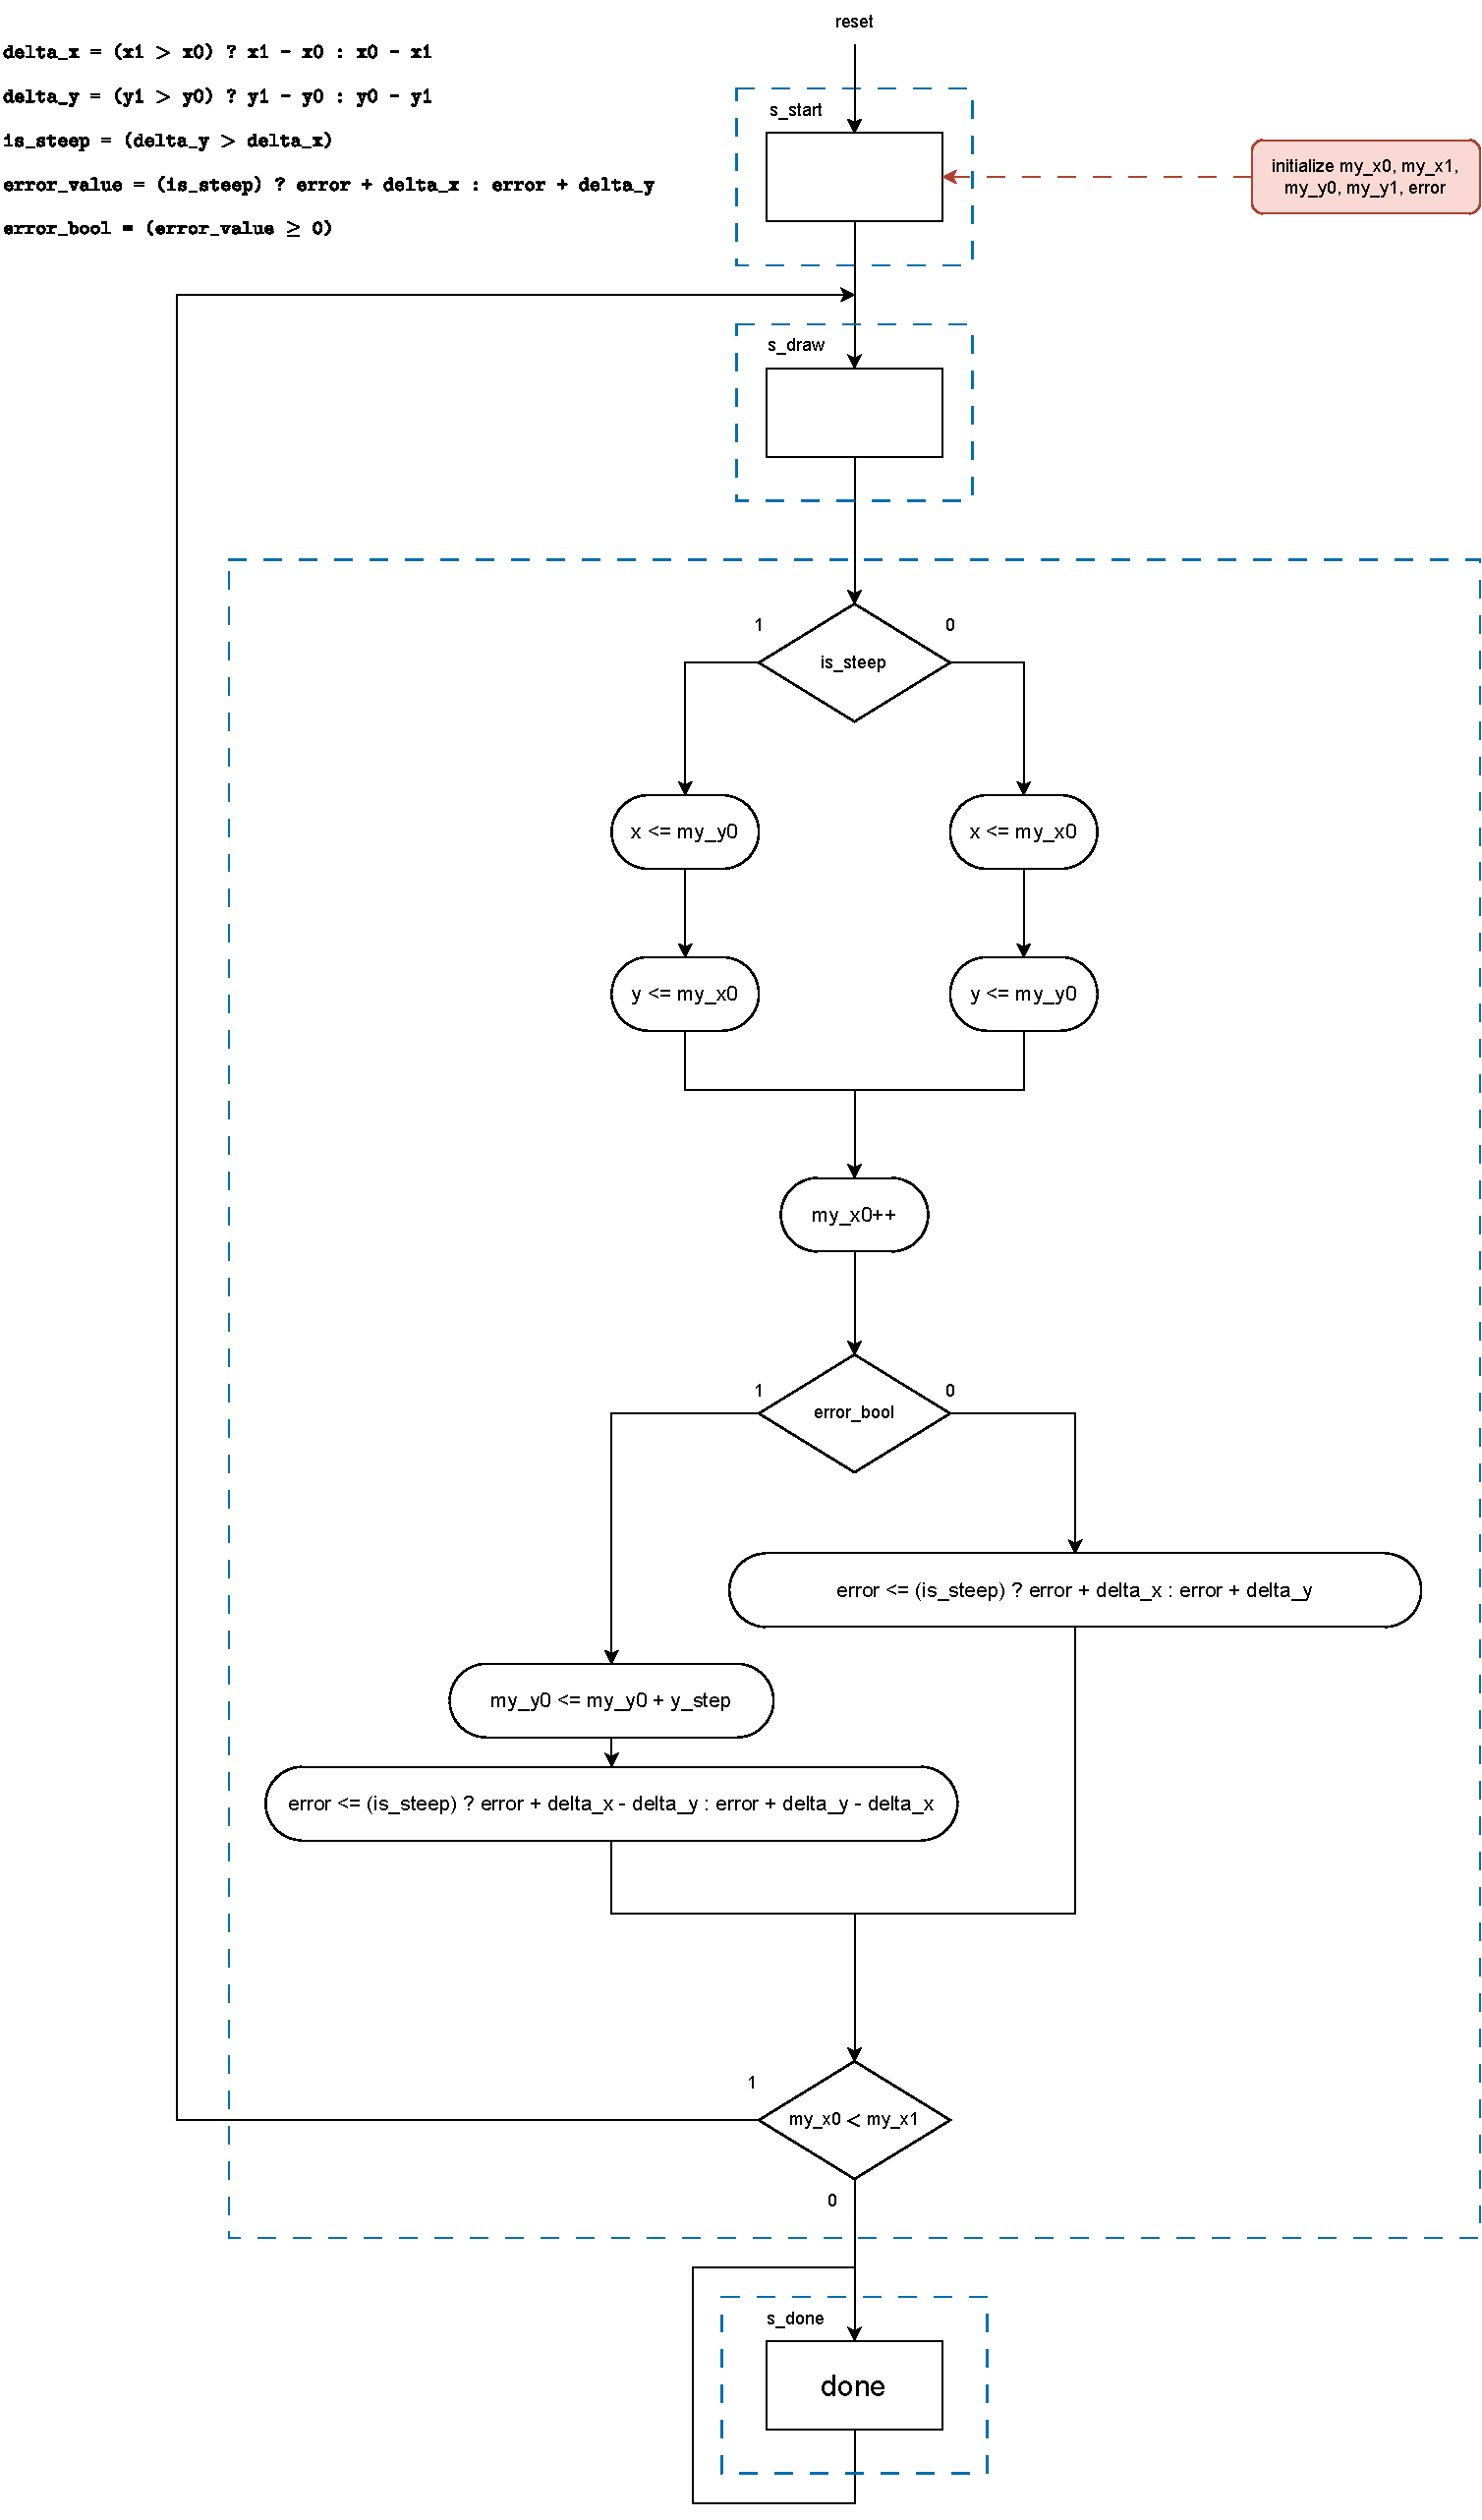
\includegraphics[scale = 0.52]{Images/line drawer diagram.pdf}
                \caption{Line Drawer ASM chart}
            \end{figure}
            
            To implement the line\_drawer module, we used the Bresenham algorithm. The system begins in the start state which sets all the values of x0, y0, x1, and y1. The values that are hard coded in the module may not be the same as the corresponding inputs. The idea our implementation runs with is that x0 is always incremented by 1 every clock cycle and y0 is only incremented when the error of y is greater than one. For example, a slope of 1/2 would wait two increments of x before y is increased because the error is finally greater than or equal to 1, the error would be (0, .50, 1) which we would then increase y. Technically if the slope of the line is less than one then the (x0, y0) and (x1, y1) values match input. If the slope of the line is greater than one, then the inputs become (y0, x0) and (y1, x1) so that y0 is now in the x place and gets increased every cycle and x0 is now responsible for incrementing when the error is greater than one. Considering the system only works when the slope is less than one, this ensures that it also works for when slope is greater than 1. A variable called is\_steep tracks this value swap and updates other parts of the code to ensure the system still works when this happens. The last case for the start is that if x0 > x1, the line goes to the left instead of the right, in this case the x0 becomes x1 and y0 becomes y1, and vice versa, then the system runs as it typically would. These conditionals and swapping of values ensure that our system works for all cases. 
            
            Once the system is in the draw state, the coordinates of the line begin to be incremented and output to the pixel buffer. The is\_steep variable described before determines if the system should use delta\_x or delta\_y to track error and updates accordingly. Then the system begins to increase x every clock cycle and y when the error is greater than 1. The swapping in the start state and the variable ensure that the entire system works regardless of the orientation of the system. Once x0 and x1 are equal or x0 is greater, the system switches to the done state. In this state it signals to the top-level controller that the line is done and the top-level then coordinates its next state.
        
        \subsection{Task \#3}
            The final step of the lab was to use the line\_drawer to make an animation of our choice. To implement our animation, we thought it would be best to provide our line\_drawer module with x0, y0, x1, y1 values output in order by a ROM. The system begins in a start state which resets the address counter and the line\_drawer module. Then it moves to the stall state for a clock cycle before moving to the “drawline” state. In the draw line state, it turns off the reset signal so the line\_drawer module can function and stays in the state until the module signals that it is done drawing the line. Then the next state of the system is the finished\_line state, which increases the count of the address accessed by the ROM and resets the line\_drawer again to prepare for the next line input. The system continues to do this until all the addresses of the ROM have been read and output, then it restarts it states.

            \begin{figure}[H]
                \centering
                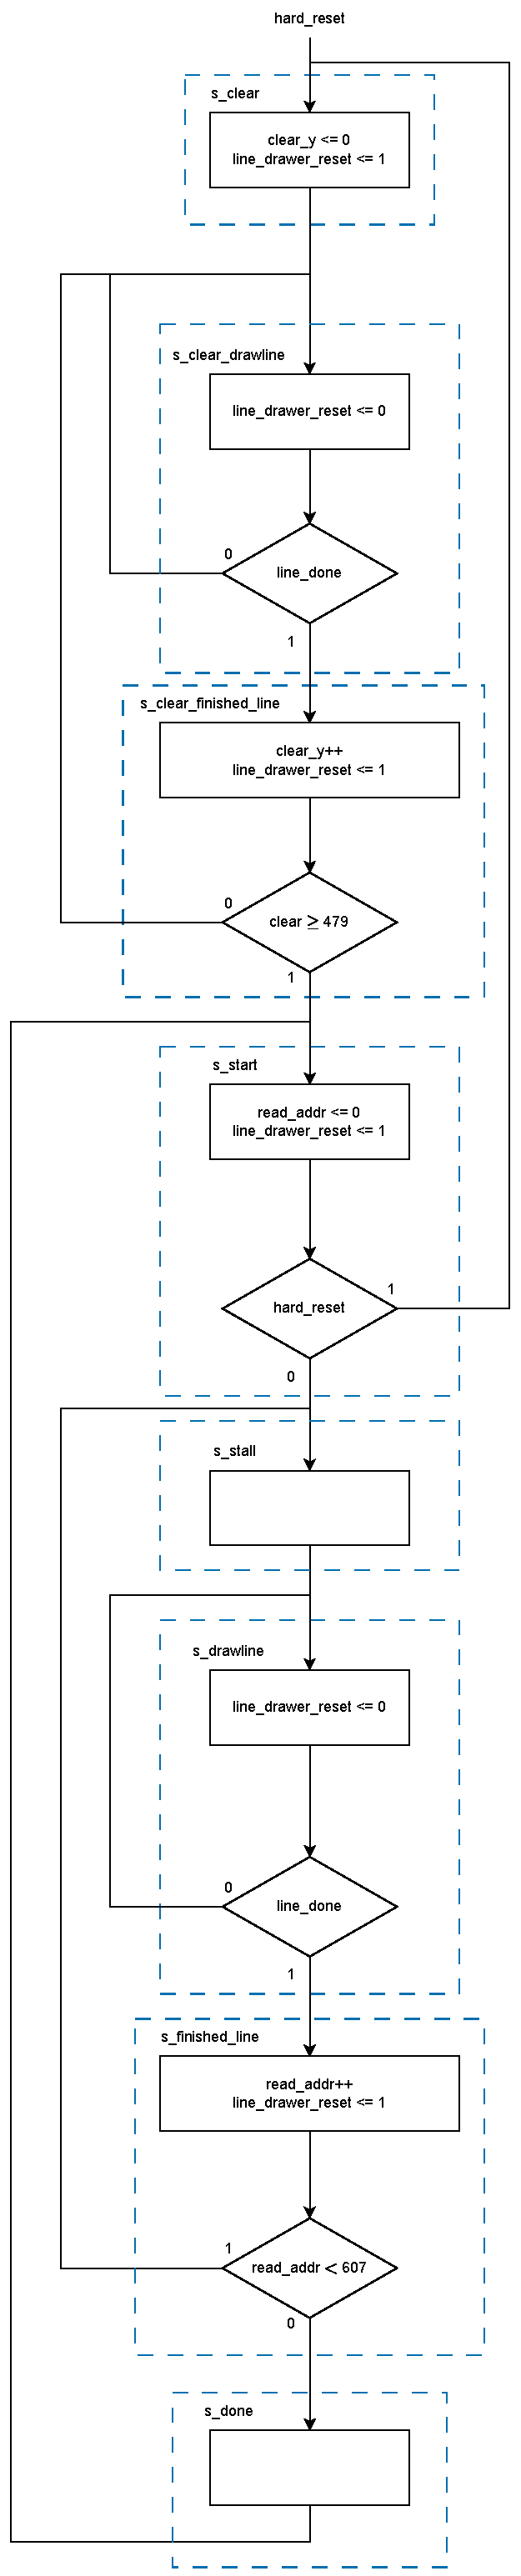
\includegraphics[scale = 0.43]{Images/top level ASM chart.pdf}
                \caption{Top Level ASM chart}
            \end{figure}

        \subsection{Overall System}
            (insert block diagram)

    \newpage
    \section{Results}
        The system we implemented in this lab has the ability to output pixel configurations to a VGA terminal as well as draw lines on the terminal to create an animation. Most of the code in this lab was provided, so we only implemented and tested two modules, the line\_drawer and the top module. However, there was not much testing of the VGA terminal output as completion of the third task could be confirmed with a simple eye-test of the final output. The only module that did require testing was the line\_drawer module. 

        \subsection{Line-Drawer Testbench}
            
            \begin{description}
                \item \textbf{Horizontal Line} \\
                    \begin{figure}[H]
                        \centering
                        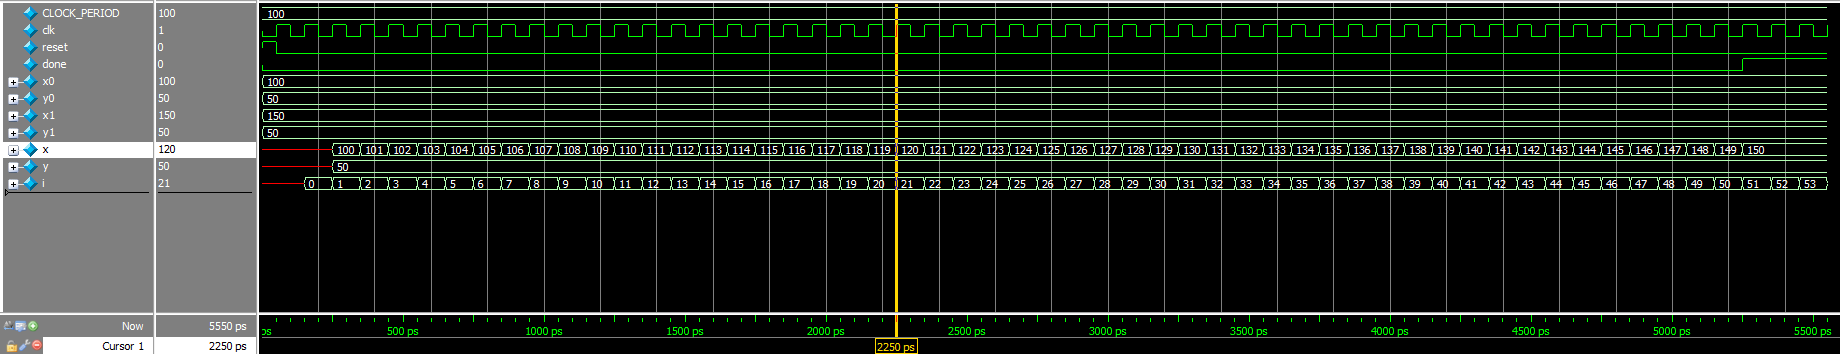
\includegraphics[scale = 0.5]{Images/horizontal line testbench.png}
                        \caption{Horizontal Line Testbench}
                    \end{figure}
                \item \textbf{Vertical Line} \\
                \item \textbf{Left-up Gradual} \\
                \item \textbf{Left-up Steep} \\
                \item \textbf{Right-up Gradual} \\
                \item \textbf{Right-up Steep} \\
                \item \textbf{Left-down Gradual} \\
                \item \textbf{Left-down Steep} \\
                \item \textbf{Right-down Gradual} \\
                \item \textbf{Right-down Steep} \\
            \end{description}

        \subsection{DE1\_SoC}
            As I stated in the section above, the top-level did not require any testing as the output could be viewed simply with an eye-test. The output that was given when we ran our system in LabsLand was the following. \\
            (add picture of animation) \\
            The animation outputs in a legible manner the word/name “CAM”.
        
        \newpage
        \subsection{Flow Summary}
            \begin{description}
                \item \textbf{DE1\_SoC} \\
                    Fitter Status : Successful - Thu Nov 16 19:05:32 2023 \\
                    Quartus Prime Version : 17.1.0 Build 590 10/25/2017 SJ  Lite Edition \\
                    Revision Name : DE1\_SoC \\
                    Top-level Entity Name : DE1\_SoC \\
                    Family : Cyclone V \\
                    Device : 5CSEMA5F31C6 \\
                    Timing Models : Final \\
                    Logic utilization (in ALMs) : 361 / 32,070 ( 1 \% ) \\
                    Total registers : 163 \\
                    Total pins : 96 / 457 ( 21 \% ) \\
                    Total virtual pins : 0 \\
                    Total block memory bits : 466,944 / 4,065,280 ( 11 \% ) \\
                    Total RAM Blocks : 58 / 397 ( 15 \% ) \\
                    Total DSP Blocks : 0 / 87 ( 0 \% ) \\
                    Total HSSI RX PCSs : 0 \\
                    Total HSSI PMA RX Deserializers : 0 \\
                    Total HSSI TX PCSs : 0 \\
                    Total HSSI PMA TX Serializers : 0 \\
                    Total PLLs : 0 / 6 ( 0 \% ) \\
                    Total DLLs : 0 / 4 ( 0 \% ) \\

                    Analysis \& Synthesis Status : Successful - Thu Nov 16 19:04:34 2023 \\
                    Quartus Prime Version : 17.1.0 Build 590 10/25/2017 SJ Lite Edition \\
                    Revision Name : DE1\_SoC \\
                    Top-level Entity Name : DE1\_SoC \\
                    Family : Cyclone V \\
                    Logic utilization (in ALMs) : N/A \\
                    Total registers : 138 \\
                    Total pins : 96 \\
                    Total virtual pins : 0 \\
                    Total block memory bits : 466,944 \\
                    Total DSP Blocks : 0 \\
                    Total HSSI RX PCSs : 0 \\
                    Total HSSI PMA RX Deserializers : 0 \\
                    Total HSSI TX PCSs : 0 \\
                    Total HSSI PMA TX Serializers : 0 \\
                    Total PLLs : 0 \\
                    Total DLLs : 0
            \end{description}
            
    \newpage
    \section{Experience Report}
        (change this)
        This lab was harder, it took a while at first to review implementations of control and datapath modules from lecture. However, once that was figured out the ASMD chart was simple to follow for the first task and generating one for task two was not too challenging either. Implementing task 2 was hard though. Figuring out timing issues with the ROM was difficult and took a significant amount of time to debug. Another challenge we encountered was trying to run the two tasks on the same board, but now that we found a method to do so the next labs we will be able to use our experience.
    

        This lab took approximately 16 hours, broken down as follows:
        \begin{description}
            \item[Reading:] 45 minutes
            \item[Design:] 15 minutes
            \item[Coding:] 7 hours
            \item[Debugging:] 5 hours
            \item[Write up:] 3 hours
        \end{description}   
        
\end{document}
